%\documentclass[twoside]{pwrthesis}


\documentclass[twoside]{iisthesis}
% --
\usepackage{polski}
\usepackage[utf8]{inputenc}
\usepackage{graphicx}

% Dodane przeze mnie d
\usepackage{fancyvrb} % dla srodowiska Verbatim
\usepackage{color}
\usepackage{lscape}

\graphicspath{{images/}}

% definicje kolorow
\definecolor{ciemnoSzary}{rgb}{0.15,0.15,0.15}
\definecolor{szary}{rgb}{0.5,0.5,0.5}
\definecolor{jasnoSzary}{rgb}{0.2,0.2,0.2}

% Konfiguracja verbatima
\fvset{
	frame=single,
	numbers=left,
	fontsize=\footnotesize,
	numbersep=12pt,
%	framerule=.5mm,
	rulecolor=\color{ciemnoSzary},
%	fillcolor=\color{jasnoSzary},
	framesep=4pt,
	stepnumber=1,
	numberblanklines=false,
	tabsize=2,
%	formatcom=\color{szary}
}

\usepackage{wrapfig}

\usepackage{mathtools}
\usepackage{enumitem}

\begin{document}

\section{Wstęp}

Celem pracy jest stworzenie systemu układającego strategię inwestycyjną za pomocą programowania genetycznego na podstawie istniejącej literatury i przedstawienie metod poprawy efektywności jego działania.


\chapter{Wprowadzenie}

\section{Heurystyczne rozwiązywanie problemów}

Przykład, prezentujący istotę heurystyki jest podany w książce L. Rutkowskiego ``Metody i techniki sztucznej inteligencji''. Zaproponowana jest sytuacja, w której ktoś zgubił szkło kontaktowe. Istnieją następujące sposoby jego szukania:

\begin{enumerate}
\item Szukanie ślepe - schylanie się i szukanie po omacku, które nie gwarantuje sukcesu.
\item Szukanie systematyczne - rozszerzanie przestrzeni rozwiązań w sposób metodyczny i zorganizowany. Gwarantuje sukces, ale jest bardzo czasochłonne.
\item Szukanie analityczne - wymaga rozwiązania równania matematycznego opisującego upadek szkła, z uwzględnieniem wszystkich czynników takich jak ruch powietrza czy siła ciążenia. Gwarantuje sukces, choć jest w praktyce niemożliwe.
\item Szukanie leniwe - polega na znalezieniu najbliższego optyka i kupieniu nowego szkła.
\item Szukanie heurystyczne - określamy przybliżony kierunek upadku i domyślamy się na jaką odległość może upaść szkło, a następnie przeszukujemy wybrany obszar. Jest to zachowanie najbardziej naturalne i najczęściej nieświadomie wybieramy właśnie taki sposób postępowania.
\end{enumerate}

Warto zauważyć, że szukanie heurystyczne wykorzystuje wiedzę o przestrzeni rozwiązań. Podejmowane są świadome decyzje o kierunku poszukiwań, możemy także ocenić aktualne postępy. Heurystyka rozwiązuje dany problem w oparciu o jakąś kreatywną metodę taką jak metoda prób i błędów lub poprzez analogię. Wyznacza ona sposób przeszukiwania przestrzeni rozwiązań, eliminując z niej te, które nie doprowadzą do rozwiązania. Heurystyka nie zawsze zapewnia dojście do rozwiązania optymalnego, jednak często nie jest to konieczne. Jeśli przegląd zupełny, czyli w podanym przykładzie szukanie systematyczne nie zwraca wyników w zadowalającym czasie, oraz niemożliwe jest wyznaczenie matematycznego opisu problemu jak we wspomnianym szukaniu analitycznym, wtedy najlepszym rozwiązaniem jest heurystyka. Nie jest to jednak naturalny sposób rozwiązywania problemów dla komputera i nie istnieją formalne dowody na skuteczność jego działania. Mimo to, w praktyce jest to najlepszy sposób na rozwiązanie niektórych problemów

Mimo, że komputery mają znacznie większe możliwości przetwarzania danych niż człowiek, niektórych problemów nie da się po prostu przeanalizować w całości. W niektórych przypadkach przestrzeń rozwiązań jest tak duża, że sprawdzenie wszystkich możliwości rozwiązań może zająć zbyt dużo czasu. Takie podejście, zwane siłowym, (lepiej znane jest określenie ``brute force'') jest proste w implementacji i wydaje się być naturalne dla komputerów.

Pierwsze naukowe próby heurystycznego rozwiązywania problemów niektórzy naukowcy \cite{history-meta} przypisują George'owi Polya. W 1945 Wydana została jego książka ``How to solve It'' \cite{polya} w której opisane były heurystyczne metody radzenia sobie z matematycznymi problemami. Polya twierdził, że problemy mogą być rozwiązywane przez ograniczony zbiór strategii, z których większość upraszcza problem. Mimo, że książka była skoncentrowana na matematycznych problemach, wiele propozycji sprawdzało się w problemach logicznych

W pracy z 1958 roku Herbert Simmon i Allen Newell \cite{simon1958heuristic}, późniejsi laureaci nagrody Turinga za badania nad sztuczną inteligencją, problemy do których należy wykorzystać podejście heurystyczne nazwali ``źle skonstruowanymi'', lub ``źle zdefiniowanymi''. Źle zdefiniowane problemy to takie, które w przeciwieństwie do dobrze skonstruowane nie mogą być wyraźnie opisane (za pomocą konkretnych liczbowych zmiennych), ich cele nie mogą być jednoznacznie zdefiniowane przez funkcję celu i do tego nie można ich rozwiązać znanymi algorytmami. 

W tym okresie pojawiły się pierwsze heurystyki rozwiązujące takie problemy, bazujące między innymi na podejściu zachłannym. Opierały się na iteratywnym wyborze najlepszej decyzji w każdym kroku działania algorytmu. Przykładami takich algorytmów jest algorytm Dijkstry do znajdowania najkrótszej ścieżki, lub algorytm Prima do znajdowania minimalnego drzewa rozpinającego \cite{Cormen:2001:IA:580470}. 

W 1970 roku Lofi Zadeh, sławny z zaproponowania matematyki rozmytej, porównywał działanie ludzkiego mózgu do działania komputerów \cite{proc-zadeh}. Mówił, że ludzki mózg operuje na niekonkretnych danych właśnie ``rozmytych pojęciach'' i potrafi wykorzystać tolerancję niepewności danych jak i rozwiązania problemu. Wtedy jednak nie potrafił tego dokonać żaden komputer. Mówił jednak, że mimo że budowa komputerów nie jest przystosowana do przetwarzania niepewnych, rozmytych danych, to jest możliwe takie zaprogramowanie go, aby takie działanie były możliwe. Wspomniał również o różnicy między tradycyjnymi obliczeniami - twardymi, które operują na konkretnych, precyzyjnych danych i obliczeniami miękkimi, które w trakcie obliczeń powinny, kiedykolwiek to możliwe, wykorzystywać tolerancję na niepewność \cite{history-soft}. 

Główne metody obliczeń miękkich rozwijały się w pewnym stopniu niezależnie od siebie. Pierwsza była wspomniana już teoria zbiorów rozmytych Lofi Zadeha. Kolejnym filarem są sieci neuronowe, które jednak były opóźniane przez małe możliwości obliczeniowe ówczesnych komputerów i dopiero ostatnio ta dziedzina nabrała prawdziwego rozpędu. Trzecim elementem są w końcu metaheurystyki.

Na początku metaheurystyki były reprezentowane jedynie przez metody ewolucyjne. Pierwszą, która zyskała uznanie była strategia ewolucyjna zaprezentowana przez Ingo Rachenberga i Hansa-Paula Schwafela \cite{Rechenberg1989}. Później L.J.Fogel opracował programowanie ewolucyjne \cite{Fogel:2011}, jednak oba podejścia były dość dalekie od dzisiejszych rozwiązań. J. Holland bazując na poprzednich pracach opracował algorytmy genetyczne \cite{Yang:2011}. Wprowadził pojęcie populacji i krzyżowania osobników. W tym okresie pojawiło się też samo pojęcie metaheurystyka. Heurystyka oznacza znajdowanie lub odkrywanie przez metody prób i błędów \cite{Yang:2011}. Dzisiaj funkcjonuje wiele definicji metaheurystyk, nie jest to pojęcie łatwe w zdefiniowaniu. Na podstawie tego, czym jest w rzeczywistości metaheurystyka powstają całe prace naukowe. Jedna z nowszych definicji została stworzona przez Freda Glovera, twórcy oryginalnej definicji oraz Kennetha Sorensena \cite{history-meta}: 

``Metaheurystyka to generyczny model algorytmiczny wysokiego poziomu który udostępnia zestaw wskazówek lub strategii do rozwoju heurystycznych algorytmów optymalizacji. Pojęcie jest również używane aby nawiązać do konkretnej implementacji heurystycznego algorytmu optymalizacji konkretnego problemu na podstawie wskazówek wyrażonych w danym modelu.''

Algorytm genetyczny znacznie zwiększył zainteresowanie naukowców metaheurystykami i w latach osiemdziesiątych i dziewięćdziesiątych powstało wiele nowych algorytmów, takich jak Tabu Search, czy Ant Colony Optimization.

\section{Algorytmy ewolucyjne}

Algorytm genetyczny został opisany przez Johna Hollanda w książce ``Adaptation in Natural and Artificial Systems''. Jego ogólny schemat jest przedstawiony na rysunku \ref{fig:schematGA}. Ewolucja naturalna jest głównym sposobem rozwiązywania problemów przez naturę. Analogicznie działa algorytm genetyczny, oraz inne bazujące na niej metaheurystyki. Podstawowe założenie jest proste - Osobniki w naturze, wraz z kolejnymi generacjami przystosowują się do środowiska w którym żyją. Przełożenie tego na algorytm może być intuicyjne.

\begin{wrapfigure}{l}{0.4\textwidth}
\caption{Ogólny schemat algorytmu genetycznego}
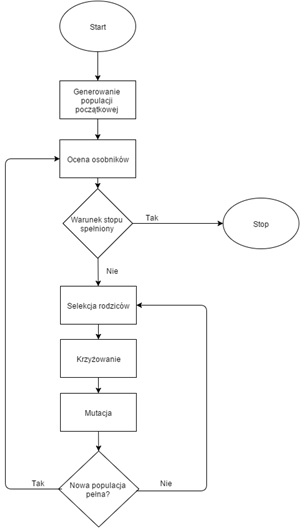
\includegraphics[width=0.4\textwidth]{schematGA.jpg}
\label{fig:schematGA}
\end{wrapfigure}

Działanie rozpoczyna się od wylosowanie populacji o pewnym rozmiarze. Populacja składa się z osobników, reprezentowanych przez zestaw cech, zwanych fenotypem. Sposób kodowanie fenotypu w pamięci nazywa się natomiast genotypem. Każdy osobnik jest oceniany, poprzez specjalną funkcję przystosowania. Następnie losowane są osobniki, które będą krzyżowały się miedzy sobą. Tak jak w naturze, większą szansę na wybór mają osobniki lepiej przystosowane, czyli takie o lepszej ocenie. Para osobników krzyżuje się, wymieniając cechami, niektóre cechy podlegają mutacji, zmieniając się losowo na inne. Proces powtarza się, póki nie zapełni się populacja nowych osobników. Każda kolejna populacja jest trochę lepsza, jednak losowa mutacja sprawia, że rozwiązanie nie utyka w lokalnym minimum. 

Osobnik może na przykład reprezentować jedno rozwiązanie problemu kolorowania grafu. Jest to często analizowany problem NP-trudny, mający także praktyczne zastosowanie. Polega na przydzieleniu wierzchołkom grafu jak najmniejszej liczby kolorów tak, aby żaden wierzchołek nie był połączony z żadnym innym o takim samym kolorze. Osobnik w tym przypadku jest reprezentowany przez wektor, którego każdy element jest reprezentuje pokolorowanie innego wierzchołka, a funkcja oceny zlicza liczbę użytych kolorów. 

Inną metaheurystyką opierającą się na analogii do ewolucji naturalnej jest programowanie genetyczne. Główną różnicą pomiędzy algorytmem ewolucyjnym jest reprezentacja osobnika.W tym przypadku osobnik jest reprezentowany przez drzewo, na którym przeprowadzane są takie sam operacje, jak w klasycznym algorytmie ewolucyjnym. Ze względu na to, że osobnik nie ma określonej wielkości, reprezentacja ta jest bardziej elastyczne. Ten zysk jest jednak równoważony przez wzrost skomplikowania.

\section{Inwestycje giełdowe}

Giełda papierów wartościowych umożliwia handel akcjami spółek, określającymi prawo do części zysków i aktywów spółki \cite{stockMarketInvestopedia}. Celem sprzedaży akcji jest pozyskanie kapitału, a inwestorzy w zamian mogą zarabiać poprzez dywidendy lub odsprzedaż akcji po wyższej cenie. Na giełdzie pracują maklerzy giełdowi, analitycy czy bankierzy inwestycyjni. Praca ich wszystkich jest związana z oceną i czasem też handlem papierami wartościowymi. Ze względu na ogromną liczbę czynników wpływających na cenę akcji, dokładne przewidzenie ruchów cen jest niemożliwe, jednak stosuje się do tego metody, które będą opisane w następnych rozdziałach. 

Historię rynków finansowych można rozpocząć w siedemnastowiecznej Holandii. W tamtych czasach zamorski handel był okraszony bardzo dużym ryzykiem, przyćmiewanym jednak przez potencjalne zyski. Aby zminimalizować ryzyko, właściciele statków mieli zwyczaj szukania inwestorów, którzy mogliby wyłożyć pieniądze na wyprawę - wyposażenie statku i załogi. W zamian otrzymywali pewien procent zysków. W siedemnastym wieku zaczęły powstawać Kompanie wschodnioindyjskie, zajmujące się handlem z daleką Azją. Pierwsza była Holenderska Kompania Wschodnioindyjska, która po raz pierwszy w historii zaoferowała kupno swoich akcji. W ten sposób sprzedawany był udział nie tylko w jednej, a we wszystkich wyprawach prowadzonych przez Kompanię. Kompanie nie dość, że proponowały znacznie większą skale przedsięwzięcia niż pojedyncze wyprawy, to dodatkowo otrzymały monopol od państwa, oferując ogromne zyski dla inwestorów.

Początkowo akcjami handlowano w kawiarniach, jednak po krótkim czasie powstały pierwsze giełdy papierów wartościowych i swoje akcje zaczęły sprzedawać Kampanie innych krajów. Korzystając ze swoich doświadczeń z giełdy holenderskiej, Joseph de la Vega opublikował w1688 roku pierwszą książkę na temat giełdy ``Confusion of Confusions''  \cite{Confusion}. Książka nie traktowała jedynie o giełdzie, a autor zamieścił w niej wiele filozoficznych przemyśleń, biblijnych, mitologicznych i historycznych aluzji. Czytelnik jest jednak zaznajamiany z historią i instrumentami giełdowymi i niektóre z zasad inwestycji przedstawionych w książce stanowi bazę dla dzisiejszych rozwiązań. 

Sposób wyboru akcji, których kupno będzie najbardziej opłacalne, nie jest prostym zadaniem. Podjęcie tej decyzji zawsze jest obarczone ryzykiem, ponieważ dokładne przewidzenie cen nie jest możliwe. Liczba czynników, które na nią wpływają jest bardzo duża, nie sposób nawet przewidzieć ich wszystkich. Dodatkowo wiele informacji trudno ocenić. Policzalne aspekty spółki, takie jak przychody, są łatwe do znalezienia. Jednak jak je ocenić w kontekście kadry zarządzającej spółką lub jej reputacji? Kombinacja trudnych w ocenie czynników czyni wybór akcji subiektywnym a nawet intuicyjnym procesem  \cite{stockPickingInvestopedia}. 

Istnieją oczywiście pewne techniki, którymi kierują się inwestorzy, a mianowicie analiza fundamentalna i analiza techniczna. Analiza fundamentalna opiera się na badaniu kondycji ekonomicznej spółki. W ocenie brane jest wiele czynników, takich jak przychody, potencjalne zyski. Analizowane jest też otoczenie spółki, jak i sektor w którym działa. Analiza fundamentalna wymaga jednak sporo wiedzy żeby wprowadzić ją w życie, szczególnie w porównaniu z analizą techniczną.

Można powiedzieć że analiza techniczna jest przeciwieństwem analizy fundamentalnej. Podczas gdy ta druga ocenia spółki na podstawie ekonomicznych danych, które obiektywnie mogą wpływać na przyszłe ceny akcji, ta pierwsza ogranicza się do analizy przeszłych cen i wolumenu akcji. ZA ojca analizy technicznej uważa się Johna J. Murphiego. W swojej książce ``Technical Analysis of the Futures Markets'', rozszerzonej następnie w ``Technical Analysis of the Financial Markets''  \cite{Murphy} opisał jej działanie i wykorzystywane narzędzia. Głównym założeniem jest stwierdzenie, że wszystkie ważne informacje szybko są odzwierciedlane w cenie akcji. Analiza techniczna opiera się na następujących podstawach:

\begin{enumerate}
\item Ceny odzwierciedlają istotne informacje. Innymi słowy, rynek jest wydajny.
\item Ceny poruszają się w trendach.
\item Historia się powtarza.
\end{enumerate}

W praktyce wykorzystywane są różne wskaźniki. Stworzone aby pomóc w identyfikacji stanów rynku i generowania odpowiednich sygnałów - kiedy jest najlepszy czas na inwestycje. Przykładem takiego wskaźnika jest średnia krocząca, czyli średnia z pewnej liczby ostatnich cen danego aktywa. W tradycyjnej analizie technicznej wykorzystywana do wygładzenia wykresu cen, często wykorzystywana w parach z różnym okresem, generując sygnały kupna lub sprzedaży podczas ich przecięcia.

Przez wiele lat giełdy papierów wartościowych były fizycznymi miejscami gdzie kupcy i sprzedawcy spotykali się i negocjowali \cite{openOutcry}. Spokojne transakcje, oko w oko w kawiarniach wyewoluowały w metodę ``open outcry''. Uczestnicy giełdy zbierali się na specjalnych arenach i krzykiem oraz specjalnymi gestami oznaczającymi parametry transakcji porozumiewali się z kontrahentami. Postępująca komputeryzacja praktycznie wyeliminowała tę formę handlu. W dzisiejszych czasach praktycznie wszystkie transakcje wykonuje się elektronicznie. Wykorzystanie komputerów dało zupełnie nowe możliwości wyboru inwestycji. 

Nie dość, że wszystkie transakcje są wykonywane przy użyciu komputerów, to jeszcze znaczna ich liczba jest wykonywana jedynie przez komputery. Za pomocą handlu algorytmicznego, wykonywana jest większość transakcji w Stanach Zjednoczonych \cite{algorythmicTradingInvestopedia}. Szczególnym elementem handu algorytmicznego jest handel wysokich częstotliwości. Opiera się na wykonywaniu bardzo szybkich i krótkich transakcji, w związku z czym jest zdominowany przez duże banki inwestycyjne i fundusze hedgingowe. Tylko one mogą pozwolić sobie na utrzymanie potrzebnej infrastruktury. Do wyboru transakcji wykorzystywane są skomplikowane algorytmy trzymane w tajemnicy. Opierają się one między innymi na zjawisku arbitrażu. Polega on na zakupie aktywa, które na jednym z rynków jest niedocenione, celem sprzedaży go na innych rynkach. Instytucje korzystający z tej metody nie konkurują jednak ze zwykłymi użytkownikami. Zwykli inwestorzy, jeśli decydują się na handel automatyczny, wykorzystują zwykle różne wskaźniki analizy technicznej, wybrane własnoręcznie lub przez algorytmy sztucznej inteligencji. Wybór analizy technicznej przy automatycznym układaniu strategii jest podyktowany głównie faktem, że wszystkie potrzebne informacje są dostępne od ręki, a jedynym problemem jest ich przetworzenie. 

Automatyczne systemy inwestycyjne mają wiele zalet ponad ręcznym inwestowaniem:

\begin{enumerate}
\item Eliminacja emocji - podczas inwestycji ludzie często kierują się emocjami. Ryzykują w końcu własne pieniądze. Zaprogramowana strategia może im pomóc podjąć decyzję, przełamać wahanie. Z drugiej strony ograniczają też inwestora, który jest skory do inwestycji przy pierwszej zauważonej okazji.
\item Możliwość backtestingu - backtesting to testowanie strategii na danych historycznych. Można w ten sposób oszacować skuteczność algorytmu, albo dobrać jego lepsze parametry.
\item Osiąganie trwałej skuteczności - Niemożliwe jest skonstruowanie strategii, która będzie za każdym razem dochodowa. Teoretycznie jednak automatyczny system inwestycyjny osiągnie stały procent korzystnych inwestycji, umożliwiając dokładniejsze zarządzanie budżetem.
\item Poprawiony czas wejścia w transakcję - komputer może zareagować w tym samym momencie, jak na rynku pojawi się konkretna sytuacja, co jest niemożliwe dla człowieka
\end{enumerate}

Do wad należy podatność na mechaniczne usterki i często konieczność posiadanie umiejętności programowania w którym z języków używanych w platformach inwestycyjnych. Co prawda istnieją programy, które umożliwiają ułożenie strategii metodą złap i przeciągnij, jednak w ten sposób działa tylko dla najprostszych strategii. 

Innym segmentem rynków finansowych jest rynek walutowy, czyli Forex (Foreign Exchange). Umożliwia on handel walutami i jest największym i najbardziej płynnym rynkiem na świecie \cite{forexInvestopedia}. Handluje się na nim wszystkimi walutami świata i dzienny obrót może przekraczać bilion dolarów. Nie dość, że możliwe jest na nim korzystanie z analizy technicznej, to posiada wiele zalet, szczególnie dla handlu automatycznego. Po pierwsze,ze względu na to, że jest to największy rynek na świecie, jest on bardzo płynny, więc możemy praktycznie w każdym momencie kupić lub sprzedać nasze aktywa po aktualnej cenie. Po drugie, jest on otwarty przez prawie cały tydzień. Zamykany jest jedynie na weekend i święta. Ogranicza to ryzyko dużych zmian cen pomiędzy zamknięciem i otwarciem handlu. Dodatkowo program inwestycyjny może działać przez większą cześć roku - giełdy papierów wartościowych. Dla porównania giełda nowojorska jest otwarta tylko sześc i pół godziny dziennie, od 9.30 do 16.00. Po trzecie, ceny transakcji są bardzo niskie, a stanowiły one duży problem w niektórych pracach w których opisane były systemy pracujące na standardowych rynkach. Kolejnym atutem, nie wykorzystywanym jednak w tej pracy jest dostęp do dużej dźwigni, dzięki czemu można osiągnąć duże zyski przy małym wkładzie własnym.

\section{Pojęcia wykorzystywane w inwestycjach}

Waluty na Forexie są grupowane w pary walutowe. Określa ona stosunek ceny pierwszej waluty z pary do drugiej. Pierwsza waluta nazywana jest \textit{bazową}, a druga \textit{kwotowaną}. Para może być ona jednak uważana za pojedynczą jednostkę, która może być kupowana i sprzedawana. Kupno danej pary oznacza kupno waluty bazowej i sprzedaż kwotowanej. Pomiędzy cenami kupna i sprzedaży jest różnica, nazywana \textit{spreadem}. Cena którą trzeba zapłacić za kupno to \textit{bid}, a za sprzedaż to \textit{ask}. Spread jest więc ceną, jaką trzeba zapłacić za przeprowadzenie transakcji.

Na giełdzie papierów wartościowych oprócz kupna akcji można również pożyczyć akcje, celem ich natychmiastowej sprzedaży i odkupienia po lepszej, niższej cenie. Rozpoczęcie takiej operacji nazywane jest \textit{krótką sprzedażą} i oznacza otwarcie \textit{krótkiej pozycji}. Analogicznie, klasyczna transakcja kupna akcji celem ich późniejszej sprzedaży nazywana jest otwarciem \textit{pozycji długiej}. Mechanizmy działania tych transakcji są ukryte przed inwestorem, ważny jest fakt, że na pozycji krótkiej zarabia się gdy cena akcji spada, a na pozycji długiej gdy cena rośnie. Pojęcia nawiązują do przekonania, że w dłuższej perspektywie czasu cena większości akcji rośnie, ze względu na rozwój spółek. Na tej obserwacji opiera się strategia buy-and-hold, czyli kup i trzymaj wykorzystywana często jako punkt odniesienia w automatycznym układaniu strategii. Polega ona na otwarciu długiej pozycji i trzymaniu jej, nie przejmując się chwilowymi spadkami cen.

Mimo że mechanizmy transakcji na Forexie są inne niż na giełdzie papierów wartościowych, wspomniane pojęcia są wykorzystywane w takim samym kontekście. Wiele badań na Forexie przeprowadzana jest na parze EUR/USD. Zwana eurodolarem, jest najbardziej płynną parą na rynku, co oznacza że zawsze można znaleźć kogoś, kto chciałby ją sprzedać po aktualnej cenie. Dodatkową zaletą tej płynności jest najmniejszy spread spośród wszystkich par.

Historyczne dane z wielu rynków są ogólnie dostępne w internecie. Mimo, że ceny walut na rynku Forex zmieniają się ciągle, niepraktyczne byłoby analizowanie każdej transakcji. Rozważa się więc ceny o różnych interwałach - np. godzinnych. Dane są wtedy dzielone na godzinne okresy, w których zawarta jest cena otwarcia (ta, z którą rozpoczął się okres), zamknięcia, minimalna i maksymalna. Często dostępny jest także \textit{wolumen}, czyli liczba aktywów które zmieniły właścicieli w danym okresie. Może ona określać stopień zainteresowania inwestorów.



\chapter{Sztuczna inteligencja w inwestycjach giełdowych}

\section{Różne podejścia w literaturze}
Ostatni przegląd metod inteligencji obliczeniowej wykorzystywanej w rynkach finansowych jest dostępny w pracy \cite{Cavalcante2016194} z 2015 roku. Zebranych jest tam wiele metod wykorzystujących głownie analizę techniczną, ale także fundamentalną. Wykorzystanie analizy technicznej sprowadza się do przetwarzania szeregów czasowych cen, czyli sekwencji cen pobranych w określonych, stałych odstępach czasu. Ze względu na to, że takie szeregi są złożone, zaszumione, dynamiczne, nieliniowe, nieparametryczne i chaotyczne \cite{Si20132581}, tradycyjne metody statystyczne nie sprawiają się zbyt dobrze, ustępując pola sztucznej inteligencji. Wykorzystywane są głównie sieci neuronowe i metaheurystyki.

Autorzy wspominają, że nie istnieje ustalona metodologia tworzenia systemów inwestycyjnych. Mimo, że prowadzone są nad tym badania, wyniki nie przedostają się do publiczności. Jest to spowodowane faktem, że jeśli komuś uda się stworzyć dobrze działający system, udostępnianie go publiczności oznaczałoby potencjalne ograniczenie własnych zysków. Celem wspomagania dalszego rozwoju, zostało wyodrębnione sześć kroków, która każda praca, opisująca system inwestycyjny powinna zawierać, opisane na rysunku \ref{fig:metodyka}.

\begin{figure}[h]
\caption{Proponowane kroki rozwoju systemu inwestycyjnego}
\centering
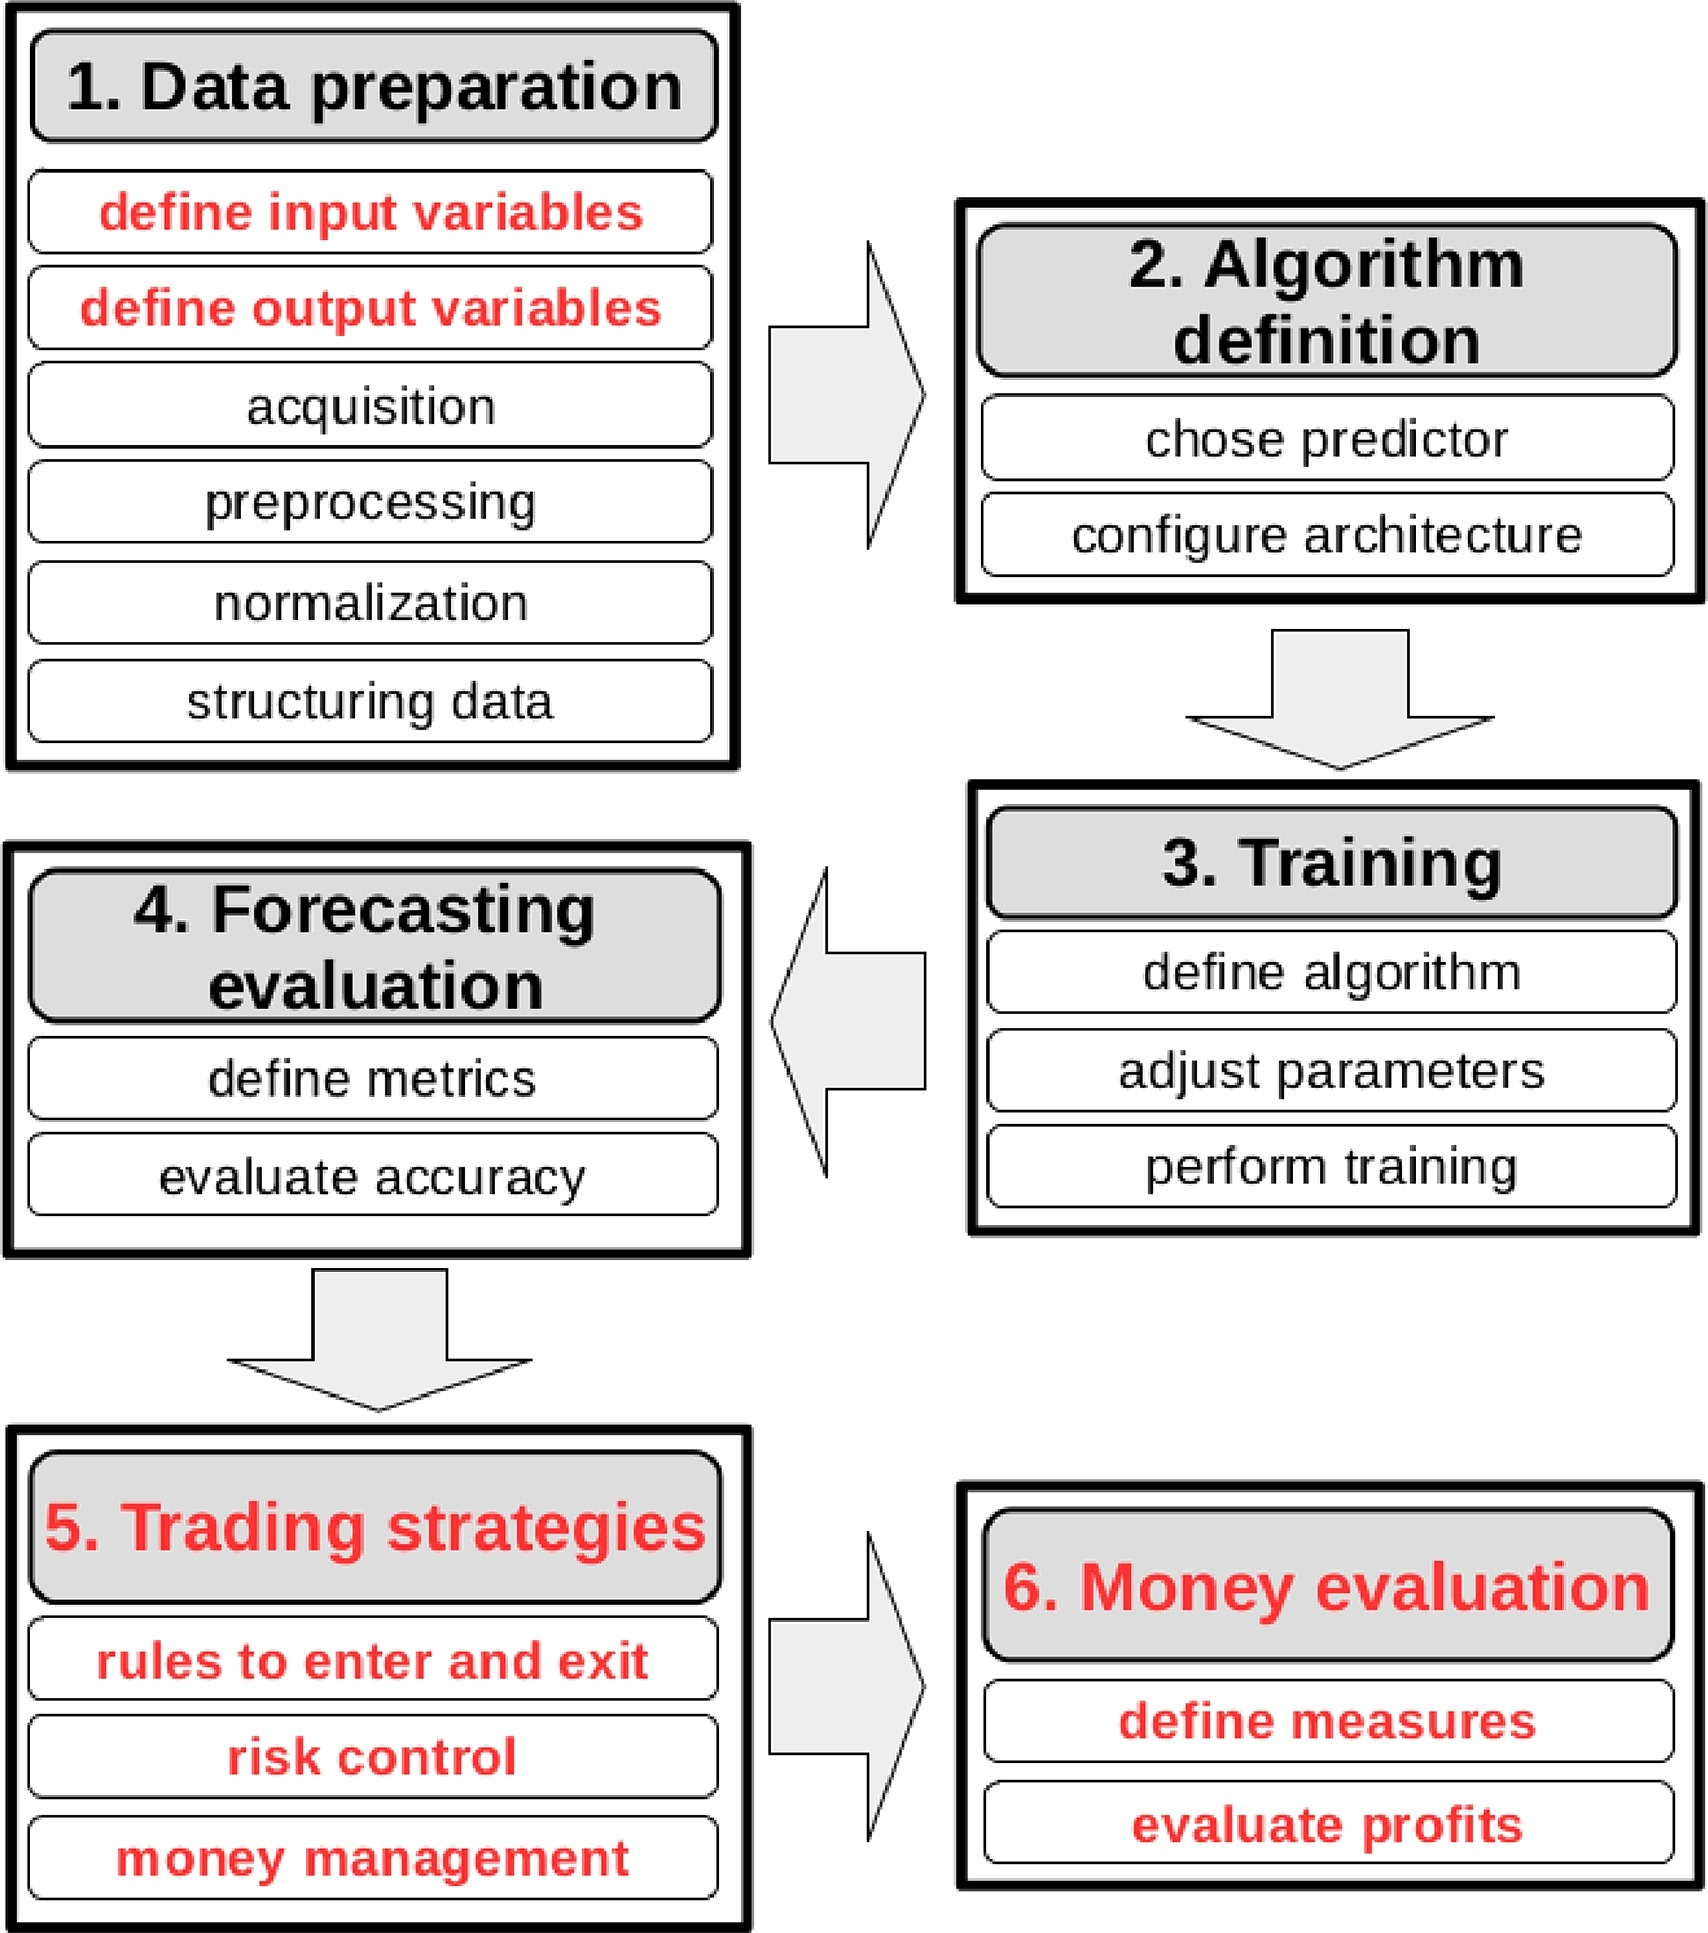
\includegraphics{metodyka.jpg}
\label{fig:metodyka}
\end{figure}

Czarne elementy można zastosować do konwencjonalnego problemu przewidywania, podczas gdy czerwone odnoszą się szczególnie do wykorzystania w rynkach finansowych. Pierwszy krok obejmuje wybór danych wejściowych i wyjściowych, pozyskanie ich i preprocessing. W przypadku analizy technicznej są to zwykle ceny lub wolumen akcji oraz różne wskaźniki techniczne, opisujące przeszłe zmiany cen. Ten krok ujawnia problem wielu metod wykorzystujących sieci neuronowe. W wielu pracach, daną wyjściową jest szansa na wzrost lub spadek ceny w kolejnym dniu. Jednak to w większości przypadków nie wystarczy do podjęcia decyzji o inwestycji.

W kolejnym drugim, trzecim i czwartym kroku wybierany jest algorytm przewidywania, uczony na wcześniej wybrany danych i oceniana jest jego skuteczność za pomocą klasycznych miar, takich jak średni błąd bezwzględny.

Kolejne, ostatnie dwa kroki odnoszą się do wykorzystania nauczonego już modelu do inwestycji. Konieczne jest takie wykorzystanie danych wyjściowych, aby w dobrym momencie kupić odpowiednie aktywa. Ważny jest mechanizm kontroli ryzyka, czyli zestaw zasad mających chronić zainwestowane pieniądze przed nagłymi stratami. Określa on, kiedy opuścić pozycję, która nie zachowuje się zgodnie z przewidywaniami. Konieczne jest także system zarządzania pieniędzmi, określający ile pieniędzy zainwestować mając pod uwagą ryzyko. Na samym końcu strategia powinna być oceniana używając backtestingu. 

Standardowym podejściem w przypadku korzystania z sieci neuronowych jest zastosowanie prostej sieci MLP, wykorzystując przedtem jakąś innowacyjną metodę przetwarzanie danych wejściowych. Proste podejście zostało opisane w pracy Dhara, Mukherjee i Ghoshala \cite{5738795}. Sieć MLP z jedną warstwą ukrytą została zastosowana do przewidywania ceny akcji na rynku Indyjskim. Na wejściu siec przyjmuje historyczne ceny otwarcia i zamknięcia oraz zwraca cenę zamknięcia następnego dnia. Sieć uczona została za pomocą algorytmu propagacji wstecznej. Przetestowane zostały różne rozmiary warstwy ukrytej i współczynniki uczenia, osiągając maksymalną skuteczność przewidywania na poziomie około 70\%. 

W innej pracy, Wang i Wang wykorzystują stochastic time strength neural network (STNN) i analizę głównych składowych. Jako dane wejściowe przyjęto dzienną cenę otwarcia, zamknięcia, minimalną i maksymalną, wolumen i dzienny obrót. Tych sześć parametrów zastało następnie przetworzone przez analizę głównych składowych, co pozwoliło zmniejszyć liczbę danych wejściowych tylko do dwóch. STNN bazuje na zwykłej MLP integrującej dodatkowo stochastyczną funkcję czasu, nadającą mniejsze wagi danym pojawiającym się dalej od teraźniejszości.

Niektóre podejścia wykorzystują także założenia analizy fundamentalnej. Nassirtoussi, Aghabozorgi, Wah i Ngo w 2015 roku \cite{KhadjehNassirtoussi2015306} wykorzystują eksploracje tekstu w nagłówkach wiadomości finansowych do przewidywania zmian cen walut na rynku Forex. Przeprowadzona jest semantyczna analiza tekstu, oraz analiza sentymentu, aby ocenić nastawienie inwestorów do wiadomości. Ważna również okazała się redukcja wymiarowości otrzymanych danych.

Autorzy przeglądu \cite{Cavalcante2016194} twierdzą, że duży potencjał, choć jeszcze niedokładnie zbadany ma wykorzystanie głębokich sieci neuronowych. Pierwsze prace wykorzystują DBL, uzyskując obiecujące wyniki. Mało czasu jest natomiast poświęcone metaheurystykom, które wykorzystywane są w trochę inny sposób.





\section{Metaheurystyki w budowaniu strategi inwestycyjnej}

Do układania strategii inwestycyjnej może być wykorzystany klasyczny algorytm ewolucyjnyi. L. Mendes, P. Godingo i J.Dias wykorzystują go w swojej pracy \cite{Mendes2012}. Mając wykształcenie ekonomiczne, skonstruowali wiele reguł, pomagając w podjęciu decyzji o inwestycji. Zmienne tych reguł, osobnych dla sygnałów kupna i sprzedaży, zostały umieszczone w wektorze, który reprezentował osobnika. Jako funkcje oceny wykorzystano \textit{współczynnik Sterlinga}. Jest to miara zwrotu z inwestycji skorygowana o ryzyko. Istnieją różne definicje tego wskaźnika ale wykorzystany został wzór:

\[\text{współczynnik Sterlinga}=\frac{\text{zysk}}{MDD}\]

Gdzie MDD (Maximum Drawdown) to maksymalna osiągnięta strata w danym czasie. Liczona jako:

\[MDD=\frac{\text{maksymalna osiągnięta wartość portfela} - \text{minimalna osiągnięta wartość portfela}}{\text{maksymalna osiągnięta wartość portfela}}\]

Ograniczenie się do otwierania tylko długich pozycji na Forexie byłoby zbyt dużym uproszczeniem. Forex wprowadza dodatkowo kolejny problem - brak jest strategii, która stanowiła by punkt odniesienia, tak jak buy-and hold w przypadku handlu akcjami. Na Forexie nie można liczyć na stały trend w którymś kierunku. Autorzy porównywali więc swoje strategie do sytuacji, gdy zysk jest zerowy. Testowano dane o różnym interwale: minutowe, pięciominutowe, piętnastominutowe oraz godzinne. Każdy interwał miał przydzielony inny okres treningowy, od miesiąca przy interwale minutowym do całego roku przy interwale godzinnym. Do każdego interwału zostały też wybrane okresy testowe o odpowiednich okresach. Brano pod uwagę parę EUR/USD i GBP/USD, jako największe, najbardziej płynne i o najmniejszym spreadzie. Osiągnięte wyniki na zbiorach treningowych były zdecydowanie pozytywne, jednak na zbiorze testowym jedynie 45\% było zyskownych na EUR/USD

Russo Vincenzo w swojej pracy magisterskiej \cite{Russo:2015} wykorzystał algorytm świetlikowy. Jest to metaheurystyka rojowa, która symuluje zachowanie robaczków świętojańskich. Optymalne wartości są znajdowane biorąc pod uwagę położenie innych świetlików, które świecą intensywniej będąc w pobliżu lepszego rozwiązania. W jego podejściu metaheurystyka miała mniejszy wpływ na strategię niż we wcześniej opisanych podejściach. Wybierała jedynie wagi pomiędzy kilkoma, wcześniej ustalonymi wskaźnikami analizy technicznej. Miała za zadanie zoptymalizować stworzony system inwestycyjny, a nie tworzyć go od podstaw. Największą zaletą takiego podejścia okazała się szybkość działania, która umożliwiała optymalizację strategii w ciągu kilku sekund, otrzymując zysku na zbiorze testowym przewyższające buy-and-hold. Sporym problemem okazały się koszty transakcji.





\section{Programowanie dynamiczne w budowaniu strategii inwestycyjnej}

Wiele prac do układania strategii inwestycyjnej na różnych rynkach wykorzystuje programowanie dynamiczne. Ma ono tą zaletę, że nie wymaga wcześniejszej wiedzy ekonomicznej czy starannego wyboru wskaźników ekonomicznych. Te zależności są wydobywane przez sam algorytm. 

Jedną z pierwszych na ten temat jest praca F. Allena i R. Karjalainena z 1999 roku \cite{Allen1999245}. We wszystkich przeszłych pracach strategie czy reguły inwestycyjne były tworzone ad hoc, co stwarzało ryzyko nadużywania danych - kierowania się nadmierną motywacją do uzyskania pozytywnego wyniku. Strategie były tworzone poprzez dopasowanie ich do posiadanych danych. Aby uniknąć tego problemu, autorzy zaproponowali użycie programowania genetycznego do układania strategii, tak aby reguły były tworzone przed użyciem danych testowych. Badania prowadzone były na indeksie S\&P 500, do którego należy 500 największych amerykańskich spółek. 

Każdy osobnik reprezentował funkcję zawartą w drzewie, każda reprezentująca osobną strategię. Drzewo jest budowane z zestawu bazowych funkcji rzeczywistych i logicznych. Każdy liść zawiera funkcję rzeczywistą, podczas gdy jego korzeniem jest funkcja logiczna. Funkcje logiczne obejmują operatory logiczne i porównania dwóch funkcji rzeczywistych. Funkcje rzeczywiste zawierają średnią kroczącą, której okres jest parametrem, oraz funkcje zwracające minimum i maksimum lokalne cen w zadanym okresie. Oprócz tego występują operatory arytmetyczne, oraz funkcja zwracająca aktualną cenę. Dodatkowo występują wartości stałe (true i false) oraz stałe wartości liczbowe. Stałe wartości logiczne są losowane na początku trenowania, tak sam jak wartości liczbowe. Podczas kolejnych generacji te wartości nie są losowane ponownie.

Ten zestaw funkcji bazowych może reprezentować strategie powszechnie wykorzystywane w inwestycjach. Przykład takich strategii jest przedstawiony na rysunku \ref{fig:allenProste}. Przy wyborze takich funkcji bazowych autorzy dodatkowo kierowali się na innych pracach, z których wynikało, że wiele skomplikowanych reguł inwestycyjnych można przedstawić korzystać z lokalnych ekstremów przeszłych cen. Średnie kroczące są wykorzystane w modelowaniu istniejących trendów cenowych. Unikano bardziej skomplikowanych reguł, przedstawianych w poprzednich badaniach, aby uniknąć ich zbytniego dopasowania do danych.

\begin{figure}[h]
\center
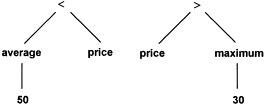
\includegraphics[width=0.4\textwidth]{AllenProste.jpg}
\label{fig:allenProste}
\caption{Osobniki programowania genetycznego reprezentujące strategie. Lewa generuje sygnał kupna, gdy średnia krocząca z 50 ostatnich cen jest mniejsza niż aktualna cena, sygnał sprzedaży w przeciwnym wypadku.}
\end{figure}

Zastosowano ciekawy sposób normalizacji danych - cena w każdym analizowanym dniu została podzielona przez 250-dniową średnią kroczącą, otrzymując ceny w okolicach jedynki. 

Jako funkcję przystosowania użyto zysku strategii ponad strategią buy-and-hold. Ze względu na to, że nie rozważano otwierania pozycji krótkich, taki wybór jest oczywisty. Wspomniano jednak o możliwości dodatkowego karania dużych spadków posiadanego kapitału, w ten sposób biorąc pod uwagę ryzyko inwestycji.

Aby właściwie przetestować zyskowność strategii, wprowadzono zbiór danych podzielono na treningowy i walidacyjny. Wszystkie operacje genetyczne było przeprowadzane na treningowym, a co generację sprawdzano, czy najlepsza otrzymana strategia jest lepsza od poprzedniej na zbiorze walidacyjnym. Tylko wtedy była ona zapamiętywana zastępując poprzednią najlepszą i ostatecznie wybierana jako najlepsza ze wszystkich generacji. Do krzyżowania wybierane były dwa osobniki, które tworzyły nowego ze swoich poddrzew. Mutacja została zaimplementowana poprzez wybór losowego drzewa jako kandydata do krzyżowania, z małym prawdopodobieństwem.

Otrzymane reguły inwestycyjne nie przynosiły stałych zysków w porównaniu do strategii buy-and-hold po odliczeniu kosztów transakcji. Mają jednak pewne zdolności przewidywania, bo opóźnienie transakcji o jeden dzień zdecydowanie pogarsza zyski.

Niedługo potem C. Nelly \cite{Neely200369} przetestował techniki kontroli ryzyka zaproponowane w poprzedniej pracy. W podejściu zmieniony został tylko sposób oceny osobników. Zastosowano między innymi wskaźnik Sharpe'a. Opracowany przez laureata Nobla Williama Sharpe'a, jest powszechnie wykorzystywany jako potencjalnego zysku w stosunku do poniesionego ryzyka. Im współczynnik jest wyższy, tym inwestycja jest bardziej atrakcyjna.

\[S=\frac{r_{p} - r_{f}}{\sigma_{p}}\]
Gdzie:
\begin{itemize}[label=]
	\item $S$: wskaźnik Sharpe'a
	\item $r_p$: średnia stopa zwrotu z inwestycji
	\item $r_f$: średnia stopa zwrotu wolna od ryzyka
	\item $\sigma_p$: odchylenie standardowe inwestycji
\end{itemize}

Inwestycją wolną od ryzyka są bony skarbowe, krótkoterminowe papiery dłużne emitowane przez rząd.

Wygenerowano strategie wykorzystując model Allena i Karjalainena z różnymi funkcjami oceny. Po zmianie funkcji oceny na wskaźnik Sharpe'a, osiągnięto trochę lepsze wyniki niż przy wcześniej zaproponowanej ocenie, jednak wciąż gorze niż strategia buy-and-hold. Powstałe strategie wykonywało mało inwestycji, upodabniając i zbliżając się do buy-and-hold, jednak nie udało się jej prześcignąć. Podobne wyniki otrzymano wykorzystując bardziej skomplikowane funkcje oceny zaczerpnięte z literatury ekonomicznej.

W pracy L. Beckera i M. Seshardi \cite{Becker:2003} udało się w końcu prześcignąć buy-and-hold. Po pierwsze, obliczenia przeprowadzano na danych miesięcznych zamiast dziennych. Celem zmiany było zredukowanie liczby inwestycji i co za tym idzie potencjalnych kosztów transakcji. Następnie zdecydowanie uproszczono reprezentację strategii. W węzłach nieterminalnych drzewa mogły pojawiać się tylko operatory logiczne (and, or, not) oraz porównania ($>$ i $<$).  W liściach mogło znaleźć się kilka różnych wskaźników technicznych:

\begin{itemize}
	\item Ceny: otwarcia, zamknięcia, maksymalna i minimalna w miesiącu
	\item Średnie kroczące: 2, 3, 4 i 10 miesięcy
	\item Rate of Change: 3 i 12 miesięcy
	\item Wskaźniki oporu ceny: 2 ostatnie minima i maksima 3-miesięcznej średniej kroczącej
	\item Wskaźniki trendu: dolna linia wyznaczona na podstawie 2 ostatnich minimów 3-miesięcznej średniej kroczącej oraz górna linia wyznaczona na podstawie 2 ostatnich maksimów 3-miesięcznej średniej kroczącej
\end{itemize}

Pierwszy eksperyment przeprowadzono z modyfikując funkcję oceny, aby oprócz zysku brała pod uwagę skomplikowanie drzewa. Większe drzewa były obarczone karą. To podejście okazało się znacznie polepszać generalizację wyników. Podczas gdy wielkość drzewa nie była ograniczana, powstałe strategie miały po kilkadziesiąt elementów.Były one praktycznie nie możliwe do zrozumienia przez człowieka. Drzewa ułożone wykorzystując zmienioną funkcje oceny, miały maksymalnie kilkanaście elementów i dodatkowo miały zdecydowanie lepsze wyniki na zbiorze testowym. Zyski na zbiorze treningowym były mniejsze, co oznaczało, że większe drzewa miały tendencję do nadmiernego dopasowania do danych uczących. 

W kolejnym eksperymencie znowu zmodyfikowano funkcję oceny. Tym razem zamiast zysku brana pod uwagę była liczba dochodowych okresów, modyfikowana również przez karę za wielkość drzewa. Średnie wyniki okazały się jeszcze lepsze niż w poprzednim eksperymencie, prawie w każdym przypadku lepsze od strategii buy-and-hold.

Kolejne polepszenie wyników uzyskano poprzez zastosowanie ewolucji kooperatywnej. W populacji istniały dwa drzewa - jedno oznaczające sygnał kupna, drugie sygnał sprzedaży. Podczas gdy oba ewoluowały w tym samym czasie w jednej populacji, każde z nich było uważane za osobny gatunek i krzyżowało się tylko ze swoim odpowiednikiem. Wykorzystując to podejście, 99,5\% otrzymanych strategii osiągało zyski większe niż buy-and-hold.

Zostały przeprowadzone dodatkowe badania nad ewolucja kooperatywną \cite{Becker03cooperativecoevolution}. Najlepsze wyniki otrzymano, gdy zamiast dwóch gatunków osobników w populacji, każdy osobnik zawierał w sobie dwa drzewa z dwoma regułami - jedną zakupu drugą sprzedaży. W tym przypadku ewaluacja osobnika jest reprezentowana przez tabelę na rysunku \ref{fig:koewolucja}. Puste pozycje oznaczają, że dana reguła nie jest brana pod uwagę w danym przypadku.

\begin{figure}[h]
\center
\caption {Podejmowanie decyzji przy osobniku reprezentowanym przez dwie reguły}
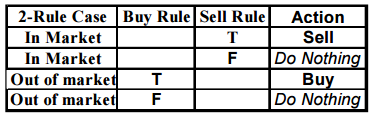
\includegraphics{koewolucja}
\label{fig:koewolucja}
\end{figure}

Ważny jest fakt, że zwiększenie kary za rozmiar drzewa gdy zwiększa się ich liczbę w osobników poprawia wyniki na zbiorze testowym. Oznacza to, że konieczne jest stałe kontrolowanie wielkości drzew, które łatwo podlegają nadmiernemu dopasowaniu do danych treningowych.

Wspomniane prace nie były jednak napisane na tyle dokładnie, aby na ich podstawie odtworzyć zaprezentowane modele. Na tym problemie skupili się D. Lohpetch i D. Corne \cite{5393324}. Oprócz dokładnego opisania wszystkich operatorów programowania genetycznego, zaproponowano nowy sposób wyboru najlepszej strategii z populacji. Podstawowe podejście polegała po prostu na wybraniu tej, która po określonej liczbie generacji miała najlepsze wyniki i testowaniu jej na zbiorze testowym. Zaproponowany sposób, mimo że autorzy tak tego nie nazwali, wprowadzał kolejny zbiór - walidacyjny, rozłączny z pozostałym treningowym i testowym. Po skończeniu ewolucji na zbiorze treningowym, najpierw ewaluowane były wszystkie strategie z finalnej populacji na zbiorze walidacyjnym i z niej wybierana była najlepszą, gotowa do następującego po nim zbioru testowego. To podejście dawało lepsze i bardziej stałe wyniki, poprzez ograniczenie dopasowania do danych treningowych.

Badania nad walidacją wyników były też przeprowadzone wcześniej przez J. Thomasa i K. Sycarę \cite{Thomas1999TheIO} na Forexie.  W badanym podejściu dane również były podzielone na 3 zbiory: treningowy, walidacyjny i testowy. Przetestowane były dwa podejścia: jedno na którym finalna populacja była testowana na zbiorze walidacyjnym i wybierana była jedna najlepsze strategia, co odpowiadało podejściu z poprzedniej pracy \cite{5393324}. W drugim na zbiór testowy kwalifikowały się wszystkie strategie, przynoszące dochód ze zbioru walidacyjnego. Mimo podobnego podejścia, autorzy otrzymali zupełnie inne wyniki. Dodatkowa walidacja okazała się pogarszać działanie powstałych strategii w każdym badanym przypadku. Wyjaśnione było to brakiem korelacji pomiędzy zbiorem walidacyjnym i testowym - wybrana strategia ze zbioru walidacyjnego nie musiała najlepiej sprawować się na testowym. Innymi słowy, nie ma korelacji pomiędzy odległością od zbioru testowego a efektywnością strategii.

Natomiast różnice pomiędzy wynikami z obu prac trudno wyjaśnić po prostu różnicami w modelu. Prawdopodobna przyczyna leży jednak w doborze danych. Być może dane na Forexie aż tak różnią się od danych z indeksu S\&P. Innym wytłumaczeniem jest dopasowanie do akurat wybranych danych. D. Lohpetch i D. Corn \cite{5393324} analizowali jedynie jeden zestaw danych treningowych i następujące po nim trzy różne zestawy zbiorów walidacyjnych i testowych różniły się tylko okresem. Podobne podejście zastosowane było w J. Thomasa i K. Sycary \cite{Thomas1999TheIO}, w którym zbiór treningowy był tylko jeden, z następującym bezpośrednio walidacyjnym i testowym.

Ciekawe podejście do wyboru danych treningowych i testowych zostało zaprezentowane w \cite{GPW}. Autor przeprowadzając badania na warszawskiej Giełdzie Papierów Wartościowych, wybrał trzy stosunkowo krótkie zbiory treningowe. Każdy przejawiał inny trend: spadkowy, neutralny lub rosnący. W taki sam sposób wybrane zostały ciągi testowe, po trzy dla każdego trendu. Podejście to korzysta z wniosków otrzymanych w poprzednio opisanej pracy,  że zbiory testowe nie muszą występować po treningowych. Otrzymane wyniki sugerowały, że strategie uczone na zbiorach spadkowych, osiągały mniejsze straty w podobnych zbiorach testowych, jednocześnie osiągając mniejsze przychody w trendach wzrostowych. Dużym problemem było duże odchylenie standardowe strategii otrzymanych po uczeniu. Oznaczało to, że algorytm miał tendencję do utykania w lokalnych minimach.

Podobny sposób wyboru zbiorów danych wykorzystane było przez P. Myszkowskiego i A. Bicza w pracy wykorzystującej programowanie genetyczne do znajdowania strategii inwestycyjnej na Forexie \cite{Bicz}. Zbadane zostały różne kombinacje zbiorów treningowych i testowych o różnych trendach. Znów ewidentna okazała się duża niestałość otrzymywanych strategii. Zaproponowane zostało podejście, które wykorzystywało tą różnorodność, tworząc jedną strategię z 200 innych. Transakcja była podejmowana tylko wtedy, gdy 60\% wszystkich strategii ze zbioru zgadzało się co do tego. Takie rozwiązanie było bardzo skuteczne, w każdym przypadku poprawiając średni wynik z otrzymanych strategii na danych zbiorach.

\section{Podsumowanie}

Wśród prac wykorzystujących programowanie genetyczne można rozróżnić dwa podejścia. Pierwsze jest skupione na ewolucji podejścia przedstawionego przez  F. Allena i R. Karjalainena\cite{Allen1999245}. Kolejne prace skupiają się głównie na uproszczeniu reprezentacji strategii, a także testowaniu potencjalnych ulepszeń. Dostępne są prace wyjaśniające niedokładnie opisane elementy algorytmu, stanowiące pewnego rodzaju poradnik do implementacji \cite{5393324}. Jednak nawet we wspomnianej pracy brakuje detali niezbędnych w odtworzeniu modelu. 

Kolejne podejście, reprezentowane przez prace P. Myszkowskiego i współautorów \cite{GPW}\cite{Bicz}, Różni się głównie reprezentacją liści drzewa. Podczas gdy w pierwszym rozwiązaniu, w liściu znajduje się wskaźnik techniczny porównany do innego wskaźnika technicznego (z których oba wcześniej ustalone), to w drugim podejściu wskaźnik techniczny jest porównany do wylosowanej liczby rzeczywistej. To rozwiązanie daje więcej wolności algorytmowi genetycznemu, poszerzając przestrzeń rozwiązań. Większa przestrzeń rozwiązań oznacza jednak potencjalnie trudniejsze strojenie algorytmu, a że oba podejścia umożliwiają otrzymanie pozytywnych wyników ( dokładne porównanie nie jest możliwe, ze względu na to że różne prace korzystają z różnych zbiorów danych, mają też inne miary sukcesu) w zastosowanym podejściu skupiono się bardziej na podejściu pierwszym. Dodatkowo, pierwsze podejście jest bardziej intuicyjne, jako że lepiej odzwierciedla sposób inwestowania ludzi. Podstawowym sygnałem wykorzystywanym przez inwestorów jest przecięcie średniej kroczącej czy to przez średnią kroczącą o innym okresie czy przez aktualną cenę. Podczas gdy jest to proste do przedstawienie w pierwszym podejściu, porównanie wartości średniej kroczącej do pewnej losowej wartości liczbowej nie daje takich możliwości.


\chapter{Zastosowane podejście}

Ze względu na niewystarczająco dokładne opisanie implementacji we wspomnianych pracach, nie było możliwe dokładne odtworzenie istniejących podejść. Zastosowany algorytm jest jednak silnie inspirowany istniejącymi rozwiązaniami, głównie pracą  D. Lohpetcha i D. Corna \cite{5393324}, która jest najnowszą i najdokładniejszą poświęconą reprezentacji zapoczątkowanej przez  F. Allena i R. Karjalainena\cite{Allen1999245}. Przy konstrukcji algorytmu brano pod uwagę wyniki i problemy i wyniki opisanych podejść. Istotna też była spójność implementacji oraz logiczne i proste przedstawienie strategii.


\section{Reprezentacja osobnika}

\begin{figure}[h]
\center
\caption {Przykładowa strategia wygenerowana przez algorytm}
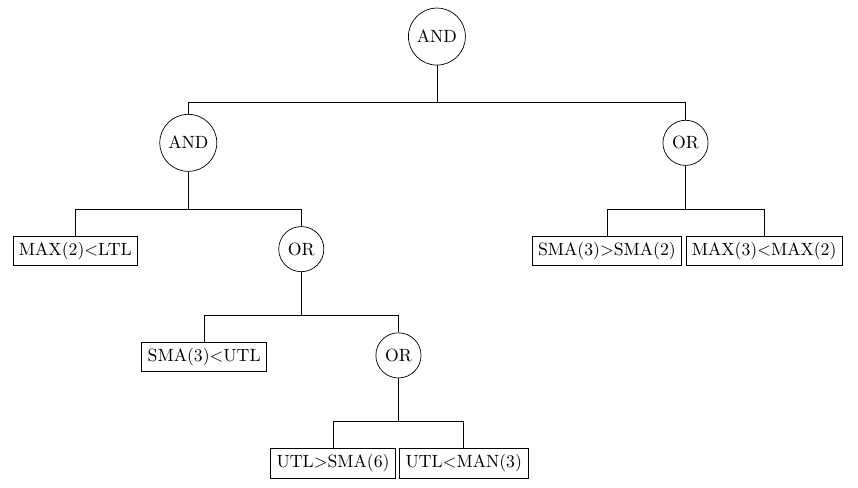
\includegraphics{drzewo}
\label{fig:drzewo}
\end{figure}

W podstawowej wersji algorytmu osobnik algorytmu genetycznego reprezentuje drzewo strategii. Przykład takiej strategii jest widoczny na rysunku \cite{fig:drzewo}. Zdecydowano się na ciągłe pozostawanie na rynku i strategie określa kiedy powinna być otwarta pozycja długa a kiedy krótka, w zależności od tego, czy drzewo zwraca wartość true czy false. Po początkowej inwestycji sprawdzane otwarta pozycja jest jedynie odwracana - z długiej na krótką i odwrotnie.

Węzły drzewa dzielą się na terminalne i nieterminalne. W węzłach nieterminalnych mogą znajdywać się operatory logiczne OR oraz AND. Zrezygnowano z operatora NOT dlatego, że nie niesie ze sobą praktycznie żadnej informacji. Ze względu na to, że w węzłach terminalnych (liściach drzewa) znajdują się porównania, operator NOT występujący przed porównaniem jedynie odwracał operator porównania, co może być przedstawione w łatwiejszy sposób.
Jak już zostało wspomniane, w liściach występuje porównanie wskaźników technicznych. Ich zestaw został zaczerpnięty z pracy \cite{5393324}, jako że był wykorzystywany już w poprzednich pracach traktujących o tym podejściu i dawał pozytywne wyniki. Dodatkowo, wybór odpowiednich wskaźników technicznych wymaga wiedzy ekonomicznej, posiadanej przez autorów wybranego zestawu:

\begin{itemize}
	\item Ceny: otwarcia, zamknięcia, maksymalna i minimalna w okresie
	\item Średnie kroczące (SMA): 2, 3, 4 i 10 ostatnich okresów
	\item Rate of Change (ROC): 3 i 12 ostatnich okresów
	\item Wskaźniki oporu ceny: 2 ostatnie minima (MAN) i maksima (MAX) średniej kroczącej z 3 ostatnich okresów
	\item Wskaźniki trendu: dolna linia wyznaczona na podstawie 2 ostatnich minimów średniej kroczącej z 3 ostatnich okresów (LTL) oraz górna linia wyznaczona na podstawie 2 ostatnich maksimów średniej kroczącej z 3 ostatnich okresów (UTL)
\end{itemize}

Adaptując zestaw z literatury została zmieniona jedynie długość okresu - ze względu na fakt, że transakcje na Forexie są obarczone mniejszym kosztem, można potencjalnie przeprowadzać ich więcej nie bojąc się o to, że cały zysk będzie przeznaczony na spłatę kosztów. Wybrano więc okresy 10-minutowe, chcąc wyuczyć system do podejmowania częstszych inwestycji.

Większość wykorzystywanych wskaźników jest prosta w implementacji. Średnia krocząca z $x$ okresów jest obliczona jako zwykła średnia arytmetyczne z $x$ ostatnich cen zamknięcia. Bardziej skomplikowany jest wskaźnik ROC:

\[ROC= \frac{P_{a} - P_{b}}{P_{a}}\]
Gdzie:
\begin{itemize}[label=]
	\item $P_a$: cena zamknięcia w okresie a
	\item $P_b$: cena zamknięcia w okresie b
\end{itemize}

ROC opisuje zmianę ceny aktywa w czasie.Jest oscylatorem, co oznacza, że jest w praktyce wykorzystywany w inny sposób niż pozostałe wskaźniki. Podczas gdy wszystkie pozostałe mogą być nałożone na wykres ceny i generować sygnały przy porównaniu ze sobą nawzajem, to oscylator przyjmuje konkretne wartości - w przypadku ROC można je ograniczyć od -1 do 1, chociaż w praktyce przedział jest zwykle mniejszy. Teoria mówi, że gdy jego wartość jest duża, może to wskazywać że cena w krótkim okresie jest zbyt duża i sugerować zmianę trendu. W wykorzystywanej literaturze nie zostało wspomniane, czy ten wskaźnik jest traktowany szczególnie. W zaimplementowanym podejściu jednak jako jedyny nie jest porównywany do pozostałych - zamiast tego, jeśli wylosowany został wskaźnik ROC jako pierwszy z porównywanej pary z liścia, to zamiast kolejnego wskaźnika losowana jest  liczba rzeczywista z zakresu -0.6 do 0.6. 

\section {Wykorzystywane dane i ocena osobnika}

\begin{figure}[h]
\center
\caption {Wykorzystywane dane}
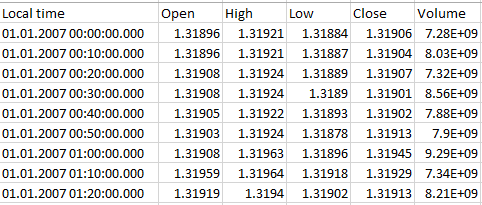
\includegraphics{data}
\label{fig:data}
\end{figure}

Wszystkie badanie przeprowadzono na Forexie, ze względu na wspomniane już zalety. Dodatkową motywacją było przetestowanie wariantu sprawdzonego już modelu na zupełnie innych danych. Dane w formacie .csv zostały pobrane z portalu Dukascopy \cite{data}. Ich początek jest widoczny na rysunku \cite{fig:data}. Można zauważyć, że w tabeli znajdują się ceny otwarcia, zamknięcia a także maksymalna i minimalna w danym okresie. 

Bardzo ważnym aspektem praktycznie nie poruszonym w literaturze jest sposób, w jaki otrzymywany jest zysk na historycznych danych. Ta wartość jest podstawą do właściwej oceny osobnika i jest niezbędna do zbudowania działającego algorytmu. W zastosowanej implementacji wzorowano się na sposobie testowania z programu MetaTrader 5 opisanym w artykule \cite{metatrader}. Metatrader jest uniwersalną platformą do handu na różnych rynkach i udostępnia zaawansowane opcje konstruowanie jak i testowania robotów handlowych - czyli programów podejmujących autonomiczne decyzje o transakcjach. 

Podstawowym podejściem jest analiza każdej zmiany ceny, czyli tak zwanego \textit{ticku}. Takie rozwiązanie wymaga jednak bardzo dużo obliczeń, ze względu na to, że cena aktywa na forexie potrafi się zmieniać bardzo szybko. Metatrader wykorzystuje więc symulację ticków. Punktem wejścia jest zestaw cen o pewnym okresie, na przykład 10 minutowym. Następnie w kolejności analizowane są ceny otwarcia, najmniejsza, największa i ostatecznie cena zamknięcia. W każdym etapie przeprowadzana jest symulacja, sprawdzane jest, czy robot powinien otworzyć jakąś pozycję. W naszym przypadku sprawdzane jest czy strategia generuje sygnał odwrócenia pozycji. Takie podejście oferuje równowagę pomiędzy dokładnością, a wymaganą mocą obliczeniową.

Konieczna była jednak jedna modyfikacja. Jeśli cena największa była za każdym razem po najmniejszej, podczas uczenia strategia była dopasowywana do tego wzorca. Dlatego kolejność ceny najmniejszej i największej była za każdym razem losowana.

Zysk liczony jest w punktach zwanych pipsami częściowymi. Pips to określenie wykorzystywane na rynku Forex, określające czwartą cyfrę po przecinku. Historycznie była to najmniejsza jednostka zmiany notowań, po prostu mniejsze zmiany nie były zapisywane. Aktualnie w popularnych parach walutowych, także w EUR/USD stosuje się pipsy częściowe, odpowiadające 1/10 zwykłego pipsa. Przyjęty sposób liczenia zysku można więc łatwo zamienić na punkty procentowe. Mimo, że ta wartość nie jest od razu przekładalna na procentowy zysk zainwestowanego kapitału, który interesuje wszystkich inwestorów, to takie podejście zostało wykorzystane we wspomnianej pracy \cite{Bicz}. Umożliwia to więc porównanie wyników i jednocześnie jest proste w implementacji.

Ważne w symulacji jest także wzięcie pod uwagę kosztów transakcji. W wykorzystywanych danych nie jest zapisany aktualny spread, który zależy od wybranego pośrednika, dlatego przyjęto stałą wartość równą 40 pipsom częściowym. Również wykorzystywana w w pracy \cite{Bicz}, przewyższa jego aktualną wartość wynoszącą około 12 pipsów częściowych. W literaturze wspomniane zostało jednak, że wyższe koszty transakcji podczas uczenia mogą powodować tworzenie bardziej ostrożnych strategii. 





















%% The Appendices part is started with the command \appendix;
%% appendix sections are then done as normal sections
%% \appendix

%% \section{}
%% \label{}

%% References
%%
%% Following citation commands can be used in the body text:
%% Usage of \cite is as follows:
%%   \cite{key}          ==>>  [#]
%%   \cite[chap. 2]{key} ==>>  [#, chap. 2]
%%   \citet{key}         ==>>  Author [#]

%% References with bibTeX database:


\bibliographystyle{iisthesis}
\bibliography{sample}

%% Authors are advised to submit their bibtex database files. They are
%% requested to list a bibtex style file in the manuscript if they do
%% not want to use model1-num-names.bst.

%% References without bibTeX database:

% \begin{thebibliography}{00}

%% \bibitem must have the following form:
%%   \bibitem{key}...
%%

% \bibitem{}

% \end{thebibliography}


\end{document}

%%
%% End of file `elsarticle-template-1-num.tex'.
